% Editable source for two_level_table.pdf, written by make_figures.py
\documentclass[border=6pt]{standalone}
\usepackage{tikz}
\usetikzlibrary{positioning,arrows.meta}
\begin{document}
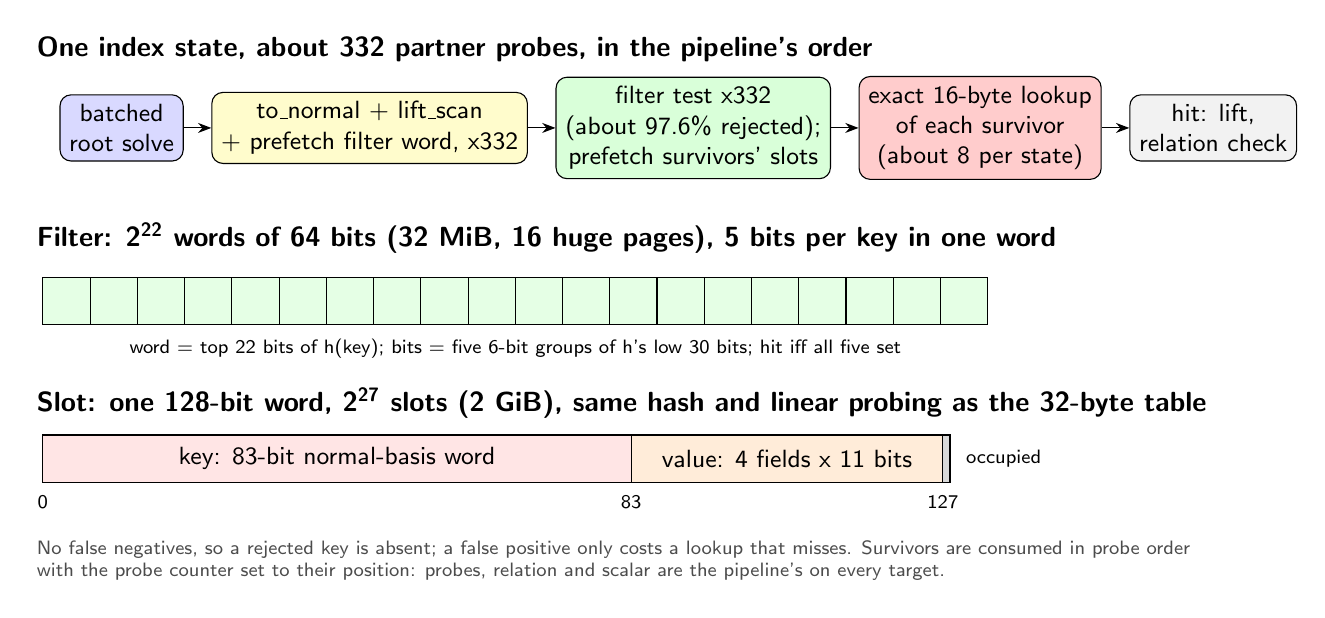
\begin{tikzpicture}[font=\sffamily\small, b/.style={draw, rounded corners, minimum height=0.8cm, align=center},
                    >={Stealth}]
\node[anchor=west,font=\sffamily\bfseries] at (-0.2,2.0) {One index state, about 332 partner probes, in the pipeline's order};
\node[b, fill=blue!15] (r) at (1.0,1.0) {batched\\root solve};
\node[b, fill=yellow!20, right=0.35 of r] (k) {to\_normal + lift\_scan\\+ prefetch filter word, x332};
\node[b, fill=green!15, right=0.35 of k] (f) {filter test x332\\(about 97.6\% rejected);\\prefetch survivors' slots};
\node[b, fill=red!20, right=0.35 of f] (l) {exact 16-byte lookup\\of each survivor\\(about 8 per state)};
\node[b, fill=black!5, right=0.35 of l] (h) {hit: lift,\\relation check};
\draw[->] (r) -- (k); \draw[->] (k) -- (f); \draw[->] (f) -- (l); \draw[->] (l) -- (h);
\node[anchor=west,font=\sffamily\bfseries] at (-0.2,-0.4) {Filter: 2\textsuperscript{22} words of 64 bits (32 MiB, 16 huge pages), 5 bits per key in one word};
\draw[fill=green!10] (0,-1.5) rectangle (12,-0.9);
\foreach \x in {0.6,1.2,...,11.4} { \draw (\x,-1.5) -- (\x,-0.9); }
\node[font=\sffamily\scriptsize] at (6,-1.8) {word = top 22 bits of h(key); bits = five 6-bit groups of h's low 30 bits; hit iff all five set};
\node[anchor=west,font=\sffamily\bfseries] at (-0.2,-2.5) {Slot: one 128-bit word, 2\textsuperscript{27} slots (2 GiB), same hash and linear probing as the 32-byte table};
\draw[fill=red!10] (0,-3.5) rectangle (7.47,-2.9) node[midway] {key: 83-bit normal-basis word};
\draw[fill=orange!15] (7.47,-3.5) rectangle (11.43,-2.9) node[midway] {value: 4 fields x 11 bits};
\draw[fill=black!15] (11.43,-3.5) rectangle (11.52,-2.9);
\node[font=\sffamily\scriptsize,anchor=west] at (11.6,-3.2) {occupied};
\node[font=\sffamily\scriptsize] at (0,-3.75) {0}; \node[font=\sffamily\scriptsize] at (7.47,-3.75) {83};
\node[font=\sffamily\scriptsize] at (11.43,-3.75) {127};
\node[anchor=west,font=\sffamily\scriptsize,text=black!70,align=left] at (-0.2,-4.5) {No false negatives, so a
rejected key is absent; a false positive only costs a lookup that misses. Survivors are consumed in probe order\\
with the probe counter set to their position: probes, relation and scalar are the pipeline's on every target.};
\end{tikzpicture}
\end{document}
